\documentclass[12pt,letterpaper]{article}
\usepackage[T1]{fontenc}
\usepackage{mathptmx}
\usepackage[letterpaper,margin=1in]{geometry}
\usepackage{amsmath,amssymb,amsfonts,amsthm,booktabs,array,microtype}
\usepackage{tikz}
\usetikzlibrary{positioning,arrows.meta,calc}
\usepackage[hidelinks]{hyperref}
\newtheorem{theorem}{Theorem}[section]
\newtheorem{proposition}[theorem]{Proposition}
\newtheorem{lemma}[theorem]{Lemma}
\newtheorem{corollary}[theorem]{Corollary}
\theoremstyle{definition}\newtheorem{definition}[theorem]{Definition}\newtheorem{example}[theorem]{Example}\newtheorem{remark}[theorem]{Remark}
\DeclareMathOperator{\agll}{AGL}\DeclareMathOperator{\pgll}{PGL}\DeclareMathOperator{\autt}{Aut}\DeclareMathOperator{\cayy}{Cay}
\title{Which $S_m$ have a complement in $S_n$?\\\large Draft 4: Corrected and expanded version}
\author{David Joyner\\\texttt{wdjoyner@gmail.com}}
\date{Original draft: 1997; revised 2007. Corrected and expanded draft: 2026}
\begin{document}\maketitle
\begin{abstract}
This corrected edition was prepared with assistance from OpenAI's ChatGPT; see the acknowledgments and separate revision log. We characterize complements to standard symmetric subgroups in terms of sharply multiply transitive permutation groups and give the resulting classification, with explicit low-degree exceptions. We also explain an exact factorization motivated by permutation storage and outline a graph-theoretic sequel involving arrangement graphs, coset graphs, and Cayley representations.
\end{abstract}
\section{Introduction}
Herbert Kociemba's question about efficient representations of Rubik's Cube permutations motivates the following finite-group problem: for which $1<m<n$ does the subgroup $S_m\leq S_n$, fixing the final $n-m$ letters pointwise, admit a complement? The original manuscript was written in 1997 and revised in 2007. This edition preserves its question and principal answer, corrects auxiliary arguments, and separates future graph-theoretic work from established results.

A subgroup $K\leq G$ is a \emph{complement} to $H\leq G$ when $G=HK$ and $H\cap K=1$. Normality is not required. Thus every $g\in G$ has a unique expression $hk$, but $G$ need not be a semidirect product. For example $S_n=A_nS_2$ for $n\geq3$, although $S_2$ is generally not normal.

\section{Literature and background}
The link between complements and sharply transitive groups is elementary permutation-group theory; standard references include Cameron \cite{Ca99} and Dixon--Mortimer \cite{DM96}. The classification of finite sharply multiply transitive groups, including the Zassenhaus theory of sharply doubly transitive groups and the exceptional Mathieu groups, is an external classification input here. The original manuscript also cited Conway--Hulpke--McKay \cite{CHM98} for transitive groups. The graph-theoretic outline in Section~\ref{sec:graphs} is new to this edition; no original classification theorem for graphs is claimed.

\subsection*{Notation}
Write $[n]=\{1,\ldots,n\}$, $S_n$ for its symmetric group, $A_n$ for the alternating group, and $C_n$ for a regular cyclic subgroup. For a finite set $X$, let
\[
X^{(k)}=\{(x_1,\ldots,x_k)\in X^k:x_i\ne x_j\ (i\ne j)\}.
\]
A permutation group is \emph{$k$-transitive} if it is transitive on $X^{(k)}$, and \emph{sharply $k$-transitive} if it acts regularly on $X^{(k)}$. In particular, a sharply $k$-transitive group of degree $n$ has order $n!/(n-k)!$.

\begin{example}
The affine transformations $x\mapsto ax+b$ of $\mathbb F_q$, with $a\ne0$, form $\agll_1(q)$, a sharply $2$-transitive group of order $q(q-1)$. The fractional linear transformations on $\mathbb P^1(\mathbb F_q)$ form $\pgll_2(q)$, sharply $3$-transitive of degree $q+1$ and order $(q+1)q(q-1)$.
\end{example}

\section{Complements and permutation actions}
We first give the general mechanism behind the classification. It is independent of the classification of finite simple groups.
\begin{lemma}\label{lem:regular}
Let $G$ act transitively on $\Omega$, and let $H=G_\alpha$ for $\alpha\in\Omega$. A subgroup $K\leq G$ complements $H$ if and only if $K$ acts regularly on $\Omega$.
\end{lemma}
\begin{proof}
The equality $G=HK$ is equivalent to transitivity of $K$: for $g\in G$, write $g=hk$ and observe that $g^{-1}\alpha=k^{-1}\alpha$; conversely, if $K$ is transitive, choose $k$ with $k^{-1}\alpha=g^{-1}\alpha$, whence $gk^{-1}\in H$. The stabilizer of $\alpha$ in $K$ is $H\cap K$. Hence transitivity together with trivial intersection is precisely regularity.
\end{proof}
\begin{proposition}\label{prop:criterion}
For $1\leq m<n$, the standard $S_m\leq S_n$ has a complement if and only if $S_n$ contains a sharply $(n-m)$-transitive subgroup of degree $n$.
\end{proposition}
\begin{proof}
Put $k=n-m$ and let $S_n$ act on $[n]^{(k)}$. The stabilizer of $(m+1,\ldots,n)$ is exactly the standard $S_m$. Apply Lemma~\ref{lem:regular}. A regular subgroup on the tuple space is precisely a sharply $k$-transitive subgroup on $[n]$.
\end{proof}
\begin{corollary}\label{cor:universal}
For every $n\geq3$, both $S_{n-1}$ and $S_2$ have complements in $S_n$, given respectively by $C_n$ and $A_n$.
\end{corollary}
\begin{proof}
The cyclic group acts regularly on $[n]$. The alternating group acts sharply $(n-2)$-transitively on $[n]$, because an even permutation is uniquely determined by the images of $n-2$ distinct letters.
\end{proof}

\subsection{Exact factorizations and induced actions}
For $G=HK$ with $H\cap K=1$, each $g$ has a unique ordered decomposition $hk$. This also implies $G=KH$ and a unique decomposition in the reverse order, but the two coordinate systems need not coincide.
\begin{proposition}\label{prop:actions}
If $G=HK$ is an exact factorization, there are homomorphisms $G\to S_K$ and $G\to S_H$ defined by
\[
R_x(k)=p_K(kx^{-1}),\qquad L_x(h)=p_H(xh),
\]
where $p_H,p_K$ denote the coordinate projections for $G=HK$ and $G=HK$, respectively.
\end{proposition}
\begin{proof}
The map $R_x$ is the action on the left coset space $H\backslash G$ induced by right multiplication by $x^{-1}$, identified with $K$ using unique representatives. Thus $R_xR_y=R_{xy}$. Similarly $L_x$ is the action on the right coset space $G/K$ induced by left multiplication, identified with $H$; hence $L_xL_y=L_{xy}$. Both are permutations and both preserve products.
\end{proof}
\begin{remark}
For more than two factors, a \emph{unique ordered factorization} means that $G_1\times\cdots\times G_r\to G$ is bijective. One may additionally require each suffix product $G_i\cdots G_r$ to be a subgroup (an iterated exact factorization). These are distinct conditions. We do not assert that products indexed by arbitrary reordered subsets are subgroups or have trivial complementary intersections.
\end{remark}

\section{Classification}\label{sec:classification}
The proof uses the standard classification of finite sharply multiply transitive permutation groups, not merely the classification of transitive overgroups. We state the precise consequence needed here as an external input; see \cite{Ca99,DM96} for the underlying theory.
\begin{theorem}[Classification input]\label{thm:input}
For a sharply $k$-transitive permutation group of degree $n$, with $2\leq k\leq n-3$, the following restrictions hold:
\begin{enumerate}
\item If $k=2$, then $n$ is a prime power.
\item If $k=3$, then $n-1$ is a prime power, or $n=10$ (the exceptional Mathieu-type action).
\item If $k=4$, then $(n,k)=(11,4)$.
\item If $k=5$, then $(n,k)=(12,5)$.
\item There are no examples with $6\leq k\leq n-3$.
\end{enumerate}
The degree-$10$ exceptional case is also covered by the projective-line construction with $q=9$; its appearance here records the exceptional isomorphism types rather than an additional degree.
\end{theorem}
\begin{remark}
The classification input is cited rather than reproved. A publication-ready version should give precise theorem/page references after checking the cited editions. The original manuscript's case-by-case order exclusions did not by themselves rule out regular subgroups of the groups considered.
\end{remark}
\begin{theorem}\label{thm:main}
Let $n>12$ and $1<m<n$. The standard subgroup $S_m$ has a complement in $S_n$ precisely when one of the following holds:
\[
m=n-1,\qquad m=2,\qquad
(m=n-2\ \text{and }n\text{ is a prime power}),
\]
\[
\text{or}\qquad (m=n-3\ \text{and }n-1\text{ is a prime power}).
\]
For $4\leq n\leq12$, the additional possibilities are given in Table~\ref{tab:small}. The cases $n\leq3$ follow directly from the definition.
\end{theorem}
\begin{proof}
By Proposition~\ref{prop:criterion}, set $k=n-m$. The cases $k=1$ and $k=n-2$ are Corollary~\ref{cor:universal}. For $k=2$, the classification input forces $n$ to be a prime power, and $\agll_1(n)$ supplies a complement. For $k=3$, the classification input forces $n-1$ to be a prime power apart from degree $10$, already of the form $9+1$; $\pgll_2(n-1)$ supplies a complement. For $4\leq k\leq n-3$ there are no degrees $n>12$ by Theorem~\ref{thm:input}. This proves the claim.
\end{proof}
\begin{table}[ht]
\centering\small
\begin{tabular}{@{}cll@{}}\toprule
$n$ & values of $m$ ($1<m<n$) & representative complements beyond $A_n,C_n$\\\midrule
4 & 2,3 & none\\
5 & 2,3,4 & $\agll_1(5)$ for $m=3$\\
6 & 2,3,5 & $\pgll_2(5)$ for $m=3$\\
7 & 2,5,6 & $\agll_1(7)$\\
8 & 2,5,6,7 & $\pgll_2(7)$; $\agll_1(8)$\\
9 & 2,6,7,8 & $\pgll_2(8)$; $\agll_1(9)$\\
10 & 2,7,9 & $\pgll_2(9)$ (also $M_{10}$) for $m=7$\\
11 & 2,7,9,10 & $M_{11}$; $\agll_1(11)$\\
12 & 2,7,9,11 & $M_{12}$; $\pgll_2(11)$\\
\bottomrule
\end{tabular}
\caption{Small degrees. Entries $m=2$ and $m=n-1$ always correspond to $A_n$ and $C_n$. The table corrects the erroneous claim in the original text that degree 10 is an additional exceptional degree outside the projective-line family.}\label{tab:small}
\end{table}
\begin{remark}\label{rem:verification}
Table~\ref{tab:small} records existence, not an exhaustive list of nonisomorphic complements. The original explicit generators have not been rerun in GAP for this revision; no computational verification is claimed.
\end{remark}
\begin{corollary}\label{cor:density}
The degrees $n$ for which there is a complement other than the universal cases $m=2,n-1$ form a set of natural density zero.
\end{corollary}
\begin{proof}
Outside finitely many exceptional degrees, such $n$ must be a prime power or one more than a prime power. The number of prime powers at most $x$ is $O(x/\log x)$, by the prime number theorem and the elementary bound on proper prime powers. Shifting by one preserves this estimate, so the set has density zero.
\end{proof}

\section{A three-factor decomposition of $S_{12}$}
The original motivation concerned the absence of a two-factor complement to $S_8$ in $S_{12}$. A three-factor decomposition provides a useful substitute.
\begin{proposition}\label{prop:12}
There are embedded subgroups $P\cong\pgll_2(11)$, $C\cong C_9$, and $H\cong S_8$ such that multiplication $P\times C\times H\to S_{12}$ is bijective.
\end{proposition}
\begin{proof}
Identify the 12 letters with $\mathbb P^1(\mathbb F_{11})$. Fix an ordered triple $(a,b,c)$ of distinct points, and let $C$ be generated by a 9-cycle on the other nine points, fixing $a,b,c$. Let $d$ be one of those nine points, and let $H$ fix $a,b,c,d$ pointwise. The group $P=\pgll_2(11)$ acts sharply transitively on ordered triples, so each ordered quadruple can be carried to $(a,b,c,e)$ by a unique element of $P$ as far as the first three coordinates are concerned. The cyclic group $C$ acts regularly on the nine choices of $e$ outside $\{a,b,c\}$. Thus the set $PC$ acts sharply transitively on ordered quadruples (using the order of factors in the action), and hence its elements are distinct modulo $H$. Finally $|P||C||H|=1320\cdot9\cdot8!=12!$. This proves bijectivity.
\end{proof}
\begin{remark}
The proof concerns a bijective three-factor multiplication map; it does not assert that $PC$ is a subgroup. This is the distinction from an iterated factorization discussed earlier.
\end{remark}

\section{Complements, regularity, and graphs}\label{sec:graphs}
This section develops the elementary graph constructions in detail, while leaving classification and spectral calculations to later drafts. Unless otherwise indicated, graphs are finite, simple, and undirected. We distinguish carefully between a regular subgroup of the natural $S_n$ action and one of the full graph automorphism group.

\subsection{Vertex stabilizers and Cayley graphs}
A graph automorphism is a permutation of the vertices preserving adjacency. A graph is \emph{vertex-transitive} if its automorphism group is transitive on vertices. For a subgroup $G\leq\autt(\Gamma)$ and a vertex $v$, write $G_v=\{g\in G:gv=v\}$.
\begin{definition}
For a finite group $K$ and an inverse-closed subset $D\subseteq K\setminus\{1\}$, the \emph{Cayley graph} $\cayy(K,D)$ has vertex set $K$ and edges $\{x,xd\}$, where $x\in K$ and $d\in D$.
\end{definition}
\begin{proposition}\label{prop:graphcriterion}
Let $G\leq\autt(\Gamma)$ be vertex-transitive and $H=G_v$. A subgroup $K\leq G$ complements $H$ if and only if $K$ acts regularly on $V(\Gamma)$. In this event $\Gamma$ is isomorphic to a Cayley graph on $K$.
\end{proposition}
\begin{proof}
The equivalence is Lemma~\ref{lem:regular}. To construct the Cayley graph, identify $x\in K$ with $x^{-1}v$ and define $D=\{d\in K:v\sim d^{-1}v\}$. The edge $x^{-1}v\sim (xd)^{-1}v$ is obtained by applying $x^{-1}$ to $v\sim d^{-1}v$ only after accounting for the order of the action: equivalently, identify $x$ with $xv$ and use edges $\{x,dx\}$, which are carried to the standard right-Cayley convention by inversion. Symmetry implies $D=D^{-1}$.
\end{proof}
\begin{remark}
The assertion that a graph is Cayley only ensures a regular subgroup of $\autt(\Gamma)$. It does not automatically give a complement inside a previously specified proper subgroup $G$.
\end{remark}
\begin{example}
The cycle $C_6$ is $\cayy(C_6,\{a,a^{-1}\})$, where $a$ generates $C_6$. Its dihedral automorphism group is vertex-transitive and contains the cyclic regular subgroup. The point stabilizer in the dihedral group has order two.
\end{example}
\begin{figure}[ht]\centering
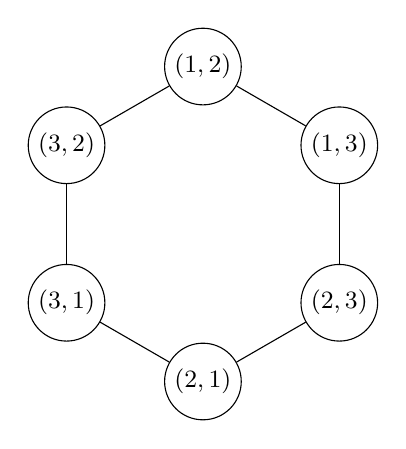
\begin{tikzpicture}[scale=1.0, every node/.style={circle,draw,fill=white,inner sep=2pt,font=\small}]
\foreach \i/\lab in {0/{(1,2)},1/{(1,3)},2/{(2,3)},3/{(2,1)},4/{(3,1)},5/{(3,2)}} {\node (v\i) at ({90-60*\i}:2) {$\lab$};}
\foreach \i in {0,...,5} {\pgfmathtruncatemacro{\j}{mod(\i+1,6)}\draw (v\i)--(v\j);}
\end{tikzpicture}
\caption{The arrangement graph $T(3,2)$ is a six-cycle. Its vertices are ordered pairs of distinct symbols.}\label{fig:t32}
\end{figure}

\subsection{Arrangement graphs}
\begin{definition}
For $1\leq k<n$, the \emph{arrangement graph} $T(n,k)$ has vertex set $[n]^{(k)}$. Two tuples are adjacent precisely when they differ in one coordinate.
\end{definition}
There are $n!/(n-k)!$ vertices. Each vertex has $k(n-k)$ neighbors, because one chooses a coordinate and replaces its entry by one of the $n-k$ symbols absent from the tuple.
\begin{proposition}\label{prop:arrangement}
If the standard $S_{n-k}$ has a complement $K$ in $S_n$, then $T(n,k)$ is a Cayley graph of $K$, with valency $k(n-k)$.
\end{proposition}
\begin{proof}
The natural action of $S_n$ on ordered tuples preserves the number of differing coordinates. Its stabilizer at the tuple $(n-k+1,\ldots,n)$ is $S_{n-k}$. Proposition~\ref{prop:graphcriterion} applies.
\end{proof}
\begin{example}
For $n=5$, $k=2$, the affine group $\agll_1(5)$ acts sharply doubly transitively on $\mathbb F_5$, hence regularly on the 20 vertices of $T(5,2)$. The graph has valency six. More explicitly, use the base tuple $(0,1)$ and write $f_{a,b}(x)=ax+b$ with $a\ne0$. Its neighbors are $(c,1)$ with $c\in\{2,3,4\}$ and $(0,c)$ with $c\in\{2,3,4\}$. For each such neighbor there is a unique affine transformation carrying $(0,1)$ to it. These six transformations form a connection set for a Cayley description, after fixing the left/right convention.
\end{example}
\begin{example}
The Mathieu group $M_{12}$ acts sharply five-transitively on 12 points. Thus $T(12,5)$ is a Cayley graph of $M_{12}$ with $12\cdot11\cdot10\cdot9\cdot8=95040$ vertices and valency $5(12-5)=35$.
\end{example}
\paragraph{Questions for a later draft.} Determine $\autt(T(n,k))$, including exceptional parameters; classify regular subgroups of the full automorphism group; and determine which Cayley representations arise from the natural $S_n$ action. The converse of Proposition~\ref{prop:arrangement} is not claimed.

\subsection{Coset graphs and double cosets}
Let $G$ act transitively on a graph, with point stabilizer $H$. Identify the vertices with the right cosets $G/H$ (written $gH$). A $G$-invariant adjacency relation is determined by the neighbors of $H$ and hence by a union $D$ of $H$-double cosets in $G$ satisfying $D=D^{-1}$ and $D\cap H=\varnothing$.
\begin{definition}
The \emph{coset graph} $\Gamma(G,H,D)$ has vertices $gH$ and edges $gH\sim g'H$ when $g^{-1}g'\in D$. Double-coset invariance makes the rule independent of coset representatives.
\end{definition}
\begin{proposition}\label{prop:coset}
If $G=KH$ and $K\cap H=1$, then every coset graph $\Gamma(G,H,D)$ is a Cayley graph of $K$.
\end{proposition}
\begin{proof}
Every left coset $gH$ has a unique representative $k\in K$. The induced $K$ action on $G/H$ is regular, and Proposition~\ref{prop:graphcriterion} applies.
\end{proof}
\begin{example}
Take $G=S_5$, $H=S_3$ fixing $(0,1)$, and $K=\agll_1(5)$. The double-coset relation corresponding to changing exactly one entry gives the arrangement graph $T(5,2)$; the same graph is a Cayley graph on $K$.
\end{example}
\begin{figure}[ht]\centering
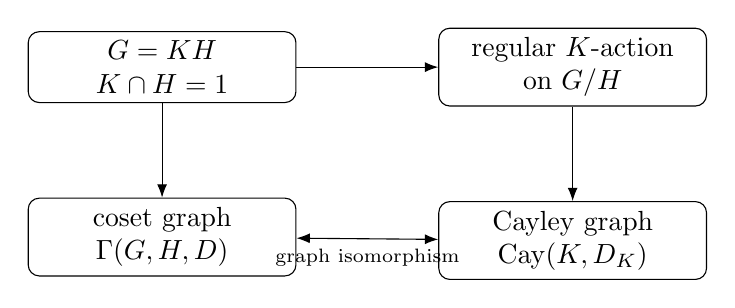
\begin{tikzpicture}[node distance=12mm and 18mm, box/.style={draw,rounded corners,align=center,minimum width=34mm,minimum height=9mm},>=Latex]
\node[box] (f) {$G=KH$\\$K\cap H=1$};
\node[box,right=of f] (r) {regular $K$-action\\on $G/H$};
\node[box,below=of r] (c) {Cayley graph\\$\cayy(K,D_K)$};
\node[box,below=of f] (d) {coset graph\\$\Gamma(G,H,D)$};
\draw[->] (f)--(r);\draw[->] (r)--(c);\draw[->] (f)--(d);\draw[<->] (d)--node[below,draw=none,font=\scriptsize]{graph isomorphism}(c);
\end{tikzpicture}
\caption{An exact factorization converts $G$-invariant coset graphs into Cayley graphs.}\label{fig:coset}
\end{figure}
\paragraph{Questions for a later draft.} Analyze connectedness (generation by $D$), arc-transitivity, and primitivity; determine which graph symmetries can be read off from subgroup factorizations.

\subsection{Johnson graphs and unordered configurations}
\begin{definition}
The \emph{Johnson graph} $J(n,k)$ has as vertices the $k$-element subsets of $[n]$. Two vertices are adjacent if they intersect in $k-1$ elements.
\end{definition}
It has $\binom nk$ vertices and valency $k(n-k)$. The stabilizer in $S_n$ of a $k$-subset is $S_k\times S_{n-k}$, unlike the pointwise stabilizer $S_{n-k}$ of an ordered tuple.
\begin{proposition}\label{prop:johnson}
A complement to $S_k\times S_{n-k}$ in $S_n$ yields a regular subgroup of the natural automorphism action on $J(n,k)$, and hence a Cayley representation.
\end{proposition}
\begin{proof}
Apply Proposition~\ref{prop:graphcriterion} to the transitive action of $S_n$ on the $k$-subsets.
\end{proof}
\begin{example}
$J(5,2)$ has ten vertices and valency six. The cyclic group $C_5$ acts transitively on the five points but cannot act regularly on the ten two-element subsets, by cardinality. Thus point-transitivity alone does not solve the Johnson complement problem.
\end{example}
\paragraph{Questions for a later draft.} Classify sharply $k$-homogeneous subgroups (regular on unordered $k$-subsets), and compare them with the sharply $k$-transitive subgroups arising from arrangement graphs. Special attention is required when $n=2k$, where complementation of subsets gives an extra graph automorphism.

\subsection{Permutation modules and adjacency spectra}
For a transitive $G$-set $G/H$, the complex permutation module is $\mathbb C[G/H]\cong\operatorname{Ind}_H^G\mathbf1$. If $K$ complements $H$, restriction to $K$ gives
\begin{equation}\label{eq:regularmodule}
\operatorname{Res}^{G}_{K}\operatorname{Ind}_{H}^{G}\mathbf1\cong\mathbb C[K],
\end{equation}
the regular representation of $K$.
\begin{proposition}\label{prop:spectrum}
For an undirected Cayley graph $\cayy(K,D)$, the adjacency operator decomposes over the irreducible complex representations $\rho$ of $K$ into blocks given by $\sum_{d\in D}\rho(d)$, with each block repeated $\dim\rho$ times (up to the left/right convention).
\end{proposition}
\begin{proof}
The adjacency operator is convolution by the indicator of $D$ on $\mathbb C[K]$. The regular representation decomposes as $\bigoplus_{\rho\in\widehat K}(\dim\rho)\rho$. Convolution preserves these isotypic summands and acts by the displayed Fourier matrices. Since $D=D^{-1}$, the operator is self-adjoint.
\end{proof}
\begin{example}
For $C_6=\langle a\rangle$ and $D=\{a,a^{-1}\}$, the six one-dimensional characters $\chi_j(a)=e^{2\pi i j/6}$ give eigenvalues $2\cos(2\pi j/6)$: $2,1,-1,-2,-1,1$.
\end{example}
\paragraph{Questions for a later draft.} Calculate explicit connection sets and Fourier blocks for $\agll_1(q)$, $\pgll_2(q)$, and the Mathieu examples. Compare the spectra associated with distinct regular groups acting on the same graph. These are proposed computations, not results asserted here.

\section{Summary and open questions}
The original complement problem is equivalent to sharply multiply transitive actions. Standard affine, projective, alternating, and exceptional Mathieu actions give the classification. The graph outline isolates three further tasks: identify full automorphism groups of arrangement graphs, classify their regular subgroups, and compare spectral decompositions coming from distinct exact factorizations. These tasks remain open within this manuscript.

\section*{Glossary}
\noindent\textbf{Arc-transitive graph}: a graph whose automorphism group is transitive on ordered adjacent vertex pairs.\par
\noindent\textbf{Arrangement graph}: graph on ordered distinct tuples with an edge for a change in exactly one coordinate.\par
\noindent\textbf{Automorphism group}: permutations of the vertices preserving adjacency.\par
\noindent\textbf{Cayley graph}: graph of a group with edges specified by an inverse-closed connection set.\par
\noindent\textbf{Complement}: subgroup $K$ satisfying $G=HK$ and $H\cap K=1$.\par
\noindent\textbf{Connection set}: the inverse-closed set of allowed group differences in a Cayley graph.\par
\noindent\textbf{Coset graph}: graph with vertices $G/H$ and adjacency prescribed by $H$-double cosets.\par
\noindent\textbf{Double coset}: subset $HgH$ of a group $G$.\par
\noindent\textbf{Exact factorization}: bijective ordered multiplication map of specified subgroup factors.\par
\noindent\textbf{Induced permutation module}: the representation $\operatorname{Ind}_H^G\mathbf1$ on the cosets $G/H$.\par
\noindent\textbf{Johnson graph}: graph on fixed-cardinality subsets adjacent when one element is exchanged.\par
\noindent\textbf{Regular action}: transitive action with trivial point stabilizers.\par
\noindent\textbf{Sharply $k$-homogeneous}: regular on unordered $k$-subsets.\par
\noindent\textbf{Sharply $k$-transitive}: regular on ordered distinct $k$-tuples.\par
\noindent\textbf{Spectrum}: multiset of eigenvalues of a graph adjacency matrix.\par
\noindent\textbf{Vertex stabilizer}: subgroup fixing a specified vertex.\par
\noindent\textbf{Vertex-transitive graph}: graph whose automorphism group is transitive on vertices.\par

\section*{Acknowledgments}
The original author thanked Herbert Kociemba for motivating correspondence and reported using GAP for selected table entries. OpenAI's ChatGPT assisted with mathematical refereeing, correction, restructuring, and drafting the graph-theoretic outline for this 2026 edition. AI review is not independent certification of the results. Details of the changes, unverified citations, and computational status appear in the separate revision log.
\begin{thebibliography}{9}
\bibitem{Ca99} P. J. Cameron, \emph{Permutation Groups}, Cambridge University Press, 1999.
\bibitem{CHM98} J. H. Conway, A. Hulpke, and J. McKay, On transitive permutation groups, \emph{LMS J. Comput. Math.} \textbf{1} (1998), 1--8.
\bibitem{DM96} J. D. Dixon and B. Mortimer, \emph{Permutation Groups}, Springer, 1996.
\bibitem{Jo97} D. Joyner, \emph{Which $S_m$ have a complement in $S_n$?}, original manuscript 1997, revised 2007.
\bibitem{Ko97} H. Kociemba, private communications with D. Joyner, 1997.
\bibitem{Ro95} J. J. Rotman, \emph{An Introduction to the Theory of Groups}, 4th ed., Springer, 1995.
\end{thebibliography}
\end{document}